\documentclass[11pt,a4paper]{article}

\usepackage[margin=2.3cm]{geometry}
\usepackage{amsmath,amssymb,amsthm}
\usepackage{booktabs}
\usepackage{array}
\usepackage{tabularx}
\usepackage{longtable}
\usepackage{verbatim}
\usepackage{listings}
\usepackage{tikz}
\usepackage{enumitem}
\usepackage{xcolor}
\usepackage{hyperref}
\usepackage{fancyhdr}
\usepackage{setspace}

\usetikzlibrary{positioning,arrows.meta}

\hypersetup{
  colorlinks=true,
  linkcolor=blue!50!black,
  urlcolor=blue!50!black,
  pdftitle={MTL458 Operating Systems --- PYQ Solutions},
  pdfauthor={MTL458}
}

\lstset{
  basicstyle=\ttfamily\small,
  breaklines=true,
  columns=fullflexible,
  frame=single,
  tabsize=4,
  keepspaces=true
}

\setlength{\headheight}{14pt}
\pagestyle{fancy}
\fancyhf{}
\lhead{MTL 458 Operating Systems}
\rhead{PYQ Solutions}
\cfoot{\thepage}

\title{\textbf{MTL 458: Operating Systems}\\[0.4em]
\large Previous Year Question Paper Solutions}
\author{IIT Delhi \and Compiled solutions for all papers in the \texttt{pyqs} folder}
\date{Papers: 2016--17, 2020--21, 2024--25}

\begin{document}
\maketitle
\tableofcontents
\newpage

\noindent\textbf{Notes.}
\begin{itemize}[leftmargin=1.2em]
  \item Every question from every paper is solved, including optional
        ``attempt any four'' and ``any two parts'' items.
  \item Each part restates the question and then gives the solution.
  \item The 2016 papers are camera scans. A few numerals were checked
        against the printed page (and, where needed, the standard
        textbook instance of the same table). In particular, Major
        2016--17 virtual addresses are \(1052\), \(2221\), \(5499\).
  \item Minor 2024--25 Q5 is solved with cache \emph{hit} rate \(95\%\)
        (miss rate then reduced to \(1\%\)).
\end{itemize}

\newpage
\section{Minor Test 1, 2016--17 (Semester 1)}

\subsection{Question 1: Program image in main memory}
\begin{quote}
\itshape
Show a layout for a program image in main memory and discuss its several
distinct sections.
\end{quote}

\textbf{Solution.}
The following is a typical virtual address-space layout of a process.  The
exact addresses and the placement of shared objects are system-dependent,
and address-space layout randomization (ASLR) deliberately varies them.

\begin{center}
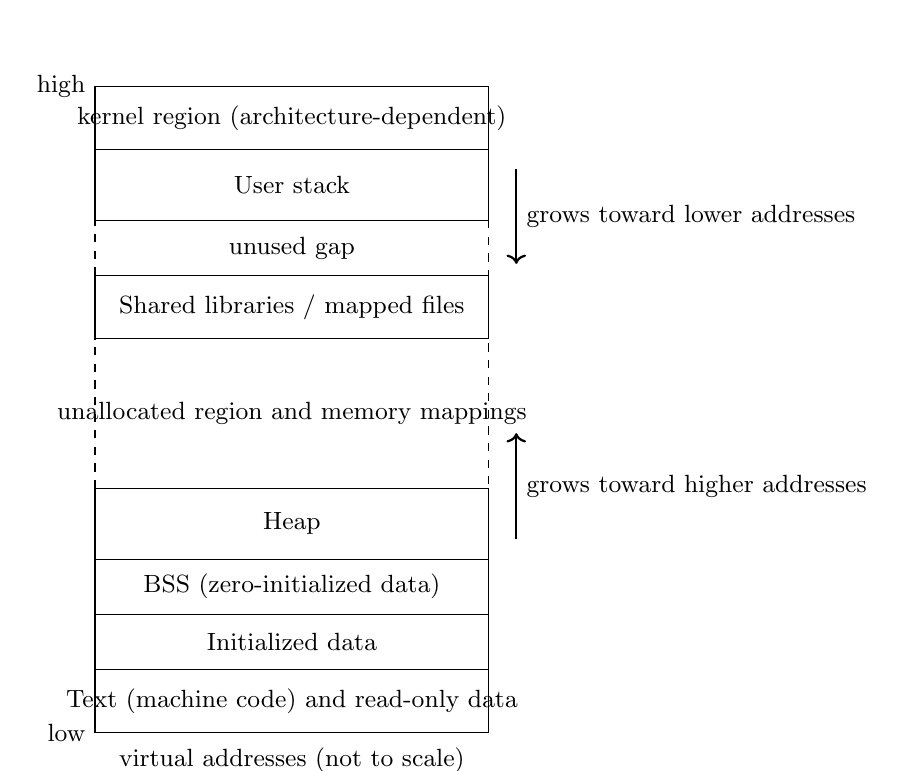
\begin{tikzpicture}[font=\small]
  \draw (0,0) rectangle (5,0.8);
  \node at (2.5,0.4) {Text (machine code) and read-only data};
  \draw (0,0.8) rectangle (5,1.5);
  \node at (2.5,1.15) {Initialized data};
  \draw (0,1.5) rectangle (5,2.2);
  \node at (2.5,1.85) {BSS (zero-initialized data)};
  \draw (0,2.2) rectangle (5,3.1);
  \node at (2.5,2.65) {Heap};
  \draw[->,thick] (5.35,2.45) -- (5.35,3.8)
      node[midway,right] {grows toward higher addresses};
  \draw[dashed] (0,3.1) rectangle (5,5.0);
  \node[align=center] at (2.5,4.05)
      {unallocated region and memory mappings};
  \draw (0,5.0) rectangle (5,5.8);
  \node at (2.5,5.4) {Shared libraries / mapped files};
  \draw[dashed] (0,5.8) rectangle (5,6.5);
  \node at (2.5,6.15) {unused gap};
  \draw (0,6.5) rectangle (5,7.4);
  \node at (2.5,6.95) {User stack};
  \draw[->,thick] (5.35,7.15) -- (5.35,5.95)
      node[midway,right] {grows toward lower addresses};
  \draw (0,7.4) rectangle (5,8.2);
  \node[align=center] at (2.5,7.8)
      {kernel region (architecture-dependent)};
  \node[left] at (0,0) {low};
  \node[left] at (0,8.2) {high};
  \node at (2.5,-0.35) {virtual addresses (not to scale)};
\end{tikzpicture}
\end{center}

\begin{itemize}
  \item \textbf{Text/code and read-only data:} This contains executable
  machine instructions and constants such as string literals.  It is
  normally readable and executable but not writable.  Because it is not
  modified, clean pages can be discarded and reloaded from the executable,
  and the same physical pages can be shared by several processes running the
  same program.

  \item \textbf{Initialized data:} Writable global and \texttt{static}
  variables having explicit nonzero initial values are stored here.  Their
  initial bytes are present in the executable file; for example,
  \texttt{static int count = 3;}.

  \item \textbf{BSS:} Writable global and \texttt{static} variables without
  an explicit initializer, or initialized to zero, belong here.  The
  executable records the required size rather than storing all the zero
  bytes; the loader supplies zero-filled memory.  For example,
  \texttt{static int table[1000];} is placed in BSS.

  \item \textbf{Heap:} This is the dynamically allocated region used by
  \texttt{malloc()} and related allocation routines.  Traditionally it
  begins after BSS and expands toward higher addresses via
  \texttt{brk}/\texttt{sbrk}; modern allocators also obtain separate
  mappings with \texttt{mmap}, particularly for large allocations.

  \item \textbf{Memory-mapping area:} Shared libraries, mapped executable
  objects, files mapped by \texttt{mmap}, and anonymous mappings are commonly
  placed between the heap and stack.  Shared library code pages may be
  physically shared while each process retains private writable state.

  \item \textbf{Stack:} The initial stack contains command-line arguments,
  the environment, and auxiliary-vector entries.  During execution it holds
  call frames, including return addresses, saved registers, parameters, and
  automatic local variables.  It conventionally grows toward lower
  addresses and is extended on demand up to a configured limit.

  \item \textbf{Kernel region:} Some architectures reserve a high part of
  the virtual address space for kernel mappings.  User-mode code cannot
  access these pages because page-table protection bits require kernel
  privilege.  On systems using kernel page-table isolation, most kernel
  mappings are absent while user code executes, but the protection principle
  is unchanged.
\end{itemize}

The address space also contains guard pages, for example below the stack, so
that an excessive growth causes a fault rather than silently corrupting
another region.  Thus, although the process appears to own one contiguous
address space, the valid regions have different permissions and need not be
contiguous in physical memory.

\subsection{Question 2: Disk I/O and running another process}
\begin{quote}
\itshape
Explain how a disk I/O request might allow the operating system to run
another process.
\end{quote}

\textbf{Solution.}
Consider process \(P_1\) executing a blocking \texttt{read()} whose requested
block is not in the page or buffer cache.

\begin{enumerate}
  \item \(P_1\) enters the kernel through a system call.  The kernel validates
  the request, creates or queues an I/O request for the disk controller, and
  arranges the destination buffer.  A controller may transfer the data by
  DMA, so the CPU need not copy each byte while the disk is operating.

  \item Because the read cannot yet return, the kernel changes \(P_1\)'s
  state from \emph{running} to \emph{waiting/blocked} on that I/O event.
  A blocked process is not eligible to use the processor.

  \item The scheduler chooses another process \(P_2\) from the ready queue.
  The OS performs a context switch: it saves \(P_1\)'s CPU state in its
  process control block (PCB), restores \(P_2\)'s saved registers and address
  space, and resumes \(P_2\).  Computation by \(P_2\) therefore overlaps the
  comparatively slow disk operation.  If no process is ready, the CPU
  executes the idle task instead.

  \item When the disk operation completes, the controller raises an
  interrupt.  The interrupt handler records completion, and the kernel wakes
  \(P_1\), moving it from the waiting queue to the ready queue.  The
  scheduler may run it immediately or later according to the scheduling
  policy.  When \(P_1\) next runs, the system call returns the data or an
  error status.
\end{enumerate}

Thus blocking I/O blocks the requesting process, not the entire processor.
The OS uses multiprogramming to keep the CPU useful during the I/O latency.
With asynchronous or nonblocking I/O, the caller itself need not block, but
the same interrupt-driven completion mechanism is normally used.

\subsection{Question 3: Creation of a new process}
\begin{quote}
\itshape
Illustrate the steps performed by an OS to create a new process.  What common
events lead to the creation of a process?
\end{quote}

\textbf{Solution.}
A process is an executing program together with an address space, CPU
context, kernel-maintained resources, and scheduling state.  A typical OS
performs the following steps:

\begin{enumerate}
  \item \textbf{Create kernel bookkeeping.} Allocate a unique process ID and
  a PCB (or task structure).  Initialize parent/child links, credentials,
  accounting data, signal state, resource limits, and the initial process
  state.

  \item \textbf{Create an address space.} Allocate page-table structures and
  virtual regions for code, data, BSS, heap, mappings, and stack.  In a
  Unix-like \texttt{fork()}, the child initially receives a logical copy of
  the parent's address space; copy-on-write allows parent and child to share
  physical pages until either writes.  When loading a new executable, as in
  \texttt{exec()}, the loader instead maps the executable's segments,
  zero-fills BSS, maps required shared libraries, and builds a fresh user
  stack containing \texttt{argv}, the environment, and auxiliary data.

  \item \textbf{Set up execution context.} Allocate a kernel stack and
  construct the saved register/trap-frame state.  Set the initial program
  counter, user stack pointer, processor mode, and other architecture state
  so that dispatch begins at the correct entry point.  After
  \texttt{fork()}, parent and child resume after the same call, but
  \texttt{fork()} returns the child's PID in the parent and \(0\) in the
  child.

  \item \textbf{Set up resources.} Establish the process's current directory,
  root directory, open-file descriptor table, terminal, signal dispositions,
  and IPC state.  A child commonly inherits references to many of these
  resources from its parent; the references, not necessarily the underlying
  objects, are copied.

  \item \textbf{Admit it for execution.} Apply admission and security checks,
  mark the process \emph{ready}, and insert it into an appropriate scheduler
  ready queue.  On a later dispatch, the scheduler restores its context and
  it begins or resumes user-mode execution.
\end{enumerate}

Unix commonly separates creation and program loading: a shell calls
\texttt{fork()} to create a child, the child calls an \texttt{exec} function
to replace its image, and the parent may call \texttt{wait()} for completion.
Other systems provide a combined \emph{spawn} operation.

Common events that cause process creation include:
\begin{itemize}
  \item \textbf{System initialization:} During boot, the kernel starts the
  initial user process, which starts services and daemons.
  \item \textbf{Interactive login or command execution:} A login service
  creates a user session and shell; the shell forks/spawns a process for a
  command or pipeline stage.
  \item \textbf{An explicit request by an existing process:} A program calls
  \texttt{fork()}, \texttt{posix\_spawn()}, or an equivalent creation API,
  for example to perform work concurrently.
  \item \textbf{Batch-job submission:} A batch scheduler admits a submitted
  job and starts one or more processes when resources become available.
  \item \textbf{A user or service request:} A server may create a worker
  process to handle a connection, print request, compilation, or other
  service operation.  Process pools are often used instead, in which case
  workers are created in advance.
\end{itemize}

\subsection{Question 4: Interleaved execution of three processes}
\begin{quote}
\itshape
Show the traces of three processes and illustrate interleaved execution
(with instruction cycles, I/O, context switch, etc.) of these processes
performed by the processor.
\end{quote}

\textbf{Solution.}
Consider three processes that are all ready at time \(0\).  Their individual
traces are
\[
\begin{array}{c@{\quad:\quad}l}
P_1 & \mathrm{CPU}(3),\ \mathrm{I/O}(4),\ \mathrm{CPU}(2),\ \mathrm{exit},\\
P_2 & \mathrm{CPU}(2),\ \mathrm{I/O}(3),\ \mathrm{CPU}(3),\ \mathrm{exit},\\
P_3 & \mathrm{CPU}(4),\ \mathrm{exit}.
\end{array}
\]
Numbers denote time units.  Assume FCFS selection of ready processes,
nonpreemptive CPU bursts, one time unit for each context switch, and that I/O
devices operate concurrently with the CPU.  One possible complete execution
is:

\begin{center}
\small
\begin{tabular}{c|l|l|l|l}
\textbf{Time} & \textbf{Processor} & \(\boldsymbol{P_1}\) &
  \(\boldsymbol{P_2}\) & \(\boldsymbol{P_3}\)\\ \hline
\(0\)--\(3\)   & execute \(P_1\) CPU burst & running & ready & ready\\
\(3\)--\(4\)   & context switch \(P_1\!\to\!P_2\) &
  blocked (I/O \(3\)--\(7\)) & selected & ready\\
\(4\)--\(6\)   & execute \(P_2\) CPU burst &
  blocked & running & ready\\
\(6\)--\(7\)   & context switch \(P_2\!\to\!P_3\) &
  blocked & blocked (I/O \(6\)--\(9\)) & selected\\
\(7\)--\(9\)   & execute \(P_3\) & ready & blocked & running\\
\(9\)--\(11\)  & execute \(P_3\) & ready & ready & running\\
\(11\)--\(12\) & context switch \(P_3\!\to\!P_1\) &
  selected & ready & terminated\\
\(12\)--\(14\) & execute \(P_1\) CPU burst &
  running & ready & terminated\\
\(14\)--\(15\) & context switch \(P_1\!\to\!P_2\) &
  terminated & selected & terminated\\
\(15\)--\(18\) & execute \(P_2\) CPU burst &
  terminated & running & terminated
\end{tabular}
\end{center}

Equivalently, the processor timeline is
\[
\underbrace{P_1}_{0\text{--}3}\;|\;
\underbrace{\mathrm{CS}}_{3\text{--}4}\;|\;
\underbrace{P_2}_{4\text{--}6}\;|\;
\underbrace{\mathrm{CS}}_{6\text{--}7}\;|\;
\underbrace{P_3}_{7\text{--}11}\;|\;
\underbrace{\mathrm{CS}}_{11\text{--}12}\;|\;
\underbrace{P_1}_{12\text{--}14}\;|\;
\underbrace{\mathrm{CS}}_{14\text{--}15}\;|\;
\underbrace{P_2}_{15\text{--}18}.
\]

Within each CPU interval, the processor repeatedly performs instruction
cycles: fetch an instruction using the current process's program counter,
decode it, execute it, and update architectural state.  At time \(3\),
\(P_1\)'s I/O instruction is realized through a system call; the OS starts
the device request and blocks \(P_1\).  During the context switch it saves
\(P_1\)'s registers, program counter, and stack pointer in its PCB and
restores those of \(P_2\).  I/O-completion interrupts at times \(7\) and \(9\)
move \(P_1\) and \(P_2\), respectively, back to the ready queue.  They resume
at the instruction following the blocking system call when later dispatched.
Thus each process observes its own sequential trace even though the single
processor interleaves their CPU bursts.  Timer preemption could produce a
finer interleaving; it is omitted here to keep the trace explicit.

\subsection{Question 5: C library wrapper and a Linux system call}
\begin{quote}
\itshape
Design a C program and show how a C library intercepts a function/statement
call along with invoking necessary system call in the Linux OS.
\end{quote}

\textbf{Solution.}
The following program writes a message to standard output using the POSIX
\texttt{write()} interface supplied by the C library.

\begin{lstlisting}[language=C]
#include <errno.h>
#include <stdio.h>
#include <unistd.h>

int main(void)
{
    const char msg[] = "Hello from user space\n";
    size_t done = 0;

    while (done < sizeof(msg) - 1) {
        ssize_t n = write(STDOUT_FILENO,
                          msg + done,
                          sizeof(msg) - 1 - done);
        if (n < 0) {
            if (errno == EINTR)
                continue;
            perror("write");
            return 1;
        }
        done += (size_t)n;
    }
    return 0;
}
\end{lstlisting}

The source-level \texttt{write()} is an ordinary user-space function call;
it is more precise to say that the C library \emph{wraps} the system call
than that it intercepts every C statement.  With dynamic linking, the call
is resolved through the executable's procedure linkage table/global offset
table to the \texttt{write} symbol in glibc.  The path is
\[
\boxed{\text{user \texttt{main}}}
\longrightarrow
\boxed{\text{glibc \texttt{write} wrapper}}
\longrightarrow
\boxed{\texttt{syscall} instruction}
\longrightarrow
\boxed{\text{Linux kernel system-call dispatcher}}
\longrightarrow
\boxed{\text{VFS/device implementation}}.
\]

On Linux for x86--64, the wrapper places the system-call number
\(\mathrm{SYS\_write}=1\) in register \texttt{rax} and the arguments
\(\texttt{fd}\), \(\texttt{buf}\), and \(\texttt{count}\) in
\texttt{rdi}, \texttt{rsi}, and \texttt{rdx}, respectively, then executes
the privileged-entry instruction \texttt{syscall}.  Other architectures use
different registers, numbers, and trap instructions.

The instruction changes control to a predefined kernel entry point and
changes privilege level; it does not create a new process.  The kernel saves
the user context, uses the system-call number to dispatch to the write
implementation, validates the file descriptor and user buffer, and sends the
request through the virtual file system to the object referenced by standard
output (for example, a terminal, pipe, or regular file).  It then returns a
result and restores user-mode execution.  A nonnegative return value is the
number of bytes accepted.  Linux kernel errors are represented internally
as negative error numbers; the glibc wrapper conventionally returns
\(-1\) and sets the thread-local variable \texttt{errno}.  The loop handles
interruption and partial writes.

For a higher-level call such as \texttt{printf()}, glibc first performs
formatting and user-space buffering.  It invokes a lower-level operation
such as \texttt{write()} only when the stream is flushed, so one
\texttt{printf()} statement does not necessarily correspond to one system
call.  The system-call boundary, not the ordinary library call itself, is
where controlled entry into the kernel occurs.

\newpage
\section{Minor Test 2, 2016--17 (Semester 1)}

\subsection*{Question 1}
\textbf{Question.}
First, give a solution (algorithm) which allows at most \(n-1\) entries in
the buffer, of the producer--consumer problem with a finite buffer.
Secondly, modify the algorithm to remedy this deficiency.

\textbf{Solution.}
Let \texttt{buffer[0..n-1]} be a circular buffer.  Initially,
\(\texttt{in}=\texttt{out}=0\).  For one producer and one consumer, the
following algorithm reserves one array position in order to distinguish
``empty'' from ``full'':

\begin{verbatim}
/* Producer */
for (;;) {
    item = produce_item();
    while ((in + 1) % n == out)
        ;                       /* full: spin */
    buffer[in] = item;
    in = (in + 1) % n;
}

/* Consumer */
for (;;) {
    while (in == out)
        ;                       /* empty: spin */
    item = buffer[out];
    out = (out + 1) % n;
    consume_item(item);
}
\end{verbatim}

Here \(\texttt{in}=\texttt{out}\) denotes an empty buffer, whereas
\((\texttt{in}+1)\bmod n=\texttt{out}\) denotes a full buffer.  Thus at
most \(n-1\) items can be stored: one physical slot is deliberately
wasted.  (With multiple producers or multiple consumers, the index
updates would additionally need mutual exclusion.)

To use all \(n\) slots, keep empty and full states separately using
counting semaphores.  Let
\[
  \texttt{mutex}=1,\qquad \texttt{empty}=n,\qquad \texttt{full}=0,
  \qquad \texttt{in}=\texttt{out}=0.
\]
The corrected bounded-buffer algorithm is:

\begin{verbatim}
/* Producer */
for (;;) {
    item = produce_item();
    sem_wait(&empty);
    sem_wait(&mutex);
    buffer[in] = item;
    in = (in + 1) % n;
    sem_post(&mutex);
    sem_post(&full);
}

/* Consumer */
for (;;) {
    sem_wait(&full);
    sem_wait(&mutex);
    item = buffer[out];
    out = (out + 1) % n;
    sem_post(&mutex);
    sem_post(&empty);
    consume_item(item);
}
\end{verbatim}

\texttt{empty} now records the number of free slots and \texttt{full}
records the number of occupied slots, so the state with
\(\texttt{full}=n\) is unambiguous.  Hence all \(n\) slots can be used.
\texttt{mutex} protects the buffer and indices, so this version also
works with multiple producers and consumers.

\subsection*{Question 2}
\textbf{Question.}
Apply the deadlock-detection algorithm to
\[
 \mathit{Available}=(2,1,0,0),
\]
\[
 \mathit{Request}=
 \begin{bmatrix}
 2&0&0&1\\
 1&0&1&0\\
 2&1&0&0
 \end{bmatrix},
 \qquad
 \mathit{Allocation}=
 \begin{bmatrix}
 0&0&1&0\\
 2&0&0&1\\
 0&1&2&0
 \end{bmatrix},
\]
and show the result.

\textbf{Solution.}
Call the three rows \(P_1,P_2,P_3\).  Initially,
\[
 \mathit{Work}=(2,1,0,0).
\]
Every process has a nonzero allocation, so initially
\(\mathit{Finish}[1]=\mathit{Finish}[2]=\mathit{Finish}[3]=\mathrm{false}\).
A vector comparison below is componentwise.

In the first scan,
\[
\begin{aligned}
 \mathit{Request}_1=(2,0,0,1)&\nleq(2,1,0,0)
       &&\text{(the fourth component fails)},\\
 \mathit{Request}_2=(1,0,1,0)&\nleq(2,1,0,0)
       &&\text{(the third component fails)},\\
 \mathit{Request}_3=(2,1,0,0)&\leq(2,1,0,0).
\end{aligned}
\]
Therefore \(P_3\) can finish and release its allocation:
\[
 \mathit{Work}
 =(2,1,0,0)+(0,1,2,0)
 =(2,2,2,0),
 \qquad \mathit{Finish}[3]=\mathrm{true}.
\]

With this new work vector, \(P_1\) still cannot finish because it needs
one unit of the fourth resource.  However,
\[
 \mathit{Request}_2=(1,0,1,0)\leq(2,2,2,0),
\]
so \(P_2\) finishes and releases its allocation:
\[
 \mathit{Work}
 =(2,2,2,0)+(2,0,0,1)
 =(4,2,2,1),
 \qquad \mathit{Finish}[2]=\mathrm{true}.
\]
Finally,
\[
 \mathit{Request}_1=(2,0,0,1)\leq(4,2,2,1),
\]
so \(P_1\) finishes:
\[
 \mathit{Work}
 =(4,2,2,1)+(0,0,1,0)
 =(4,2,3,1),
 \qquad \mathit{Finish}[1]=\mathrm{true}.
\]
Thus a complete finishing sequence is
\[
 \boxed{P_3,\ P_2,\ P_1}.
\]
All \(\mathit{Finish}\) entries become true; therefore no process is
deadlocked.

\subsection*{Question 3}
\textbf{Question.}
Suppose there are two types of philosophers.  A ``lefty'' always picks
up the left fork first, while a ``righty'' always picks up the right
fork first.  Using semaphores, define both types of philosophers'
behaviour.

\textbf{Solution.}
Number the \(N\) philosophers and forks from \(0\) to \(N-1\).  For
philosopher \(i\), define
\[
  \mathit{left}(i)=i,\qquad
  \mathit{right}(i)=(i+1)\bmod N.
\]
Each \texttt{fork[i]} is a binary semaphore initialized to \(1\).

\begin{verbatim}
void lefty(int i)
{
    int left  = i;
    int right = (i + 1) % N;

    for (;;) {
        think();
        sem_wait(&fork[left]);
        sem_wait(&fork[right]);
        eat();
        sem_post(&fork[right]);
        sem_post(&fork[left]);
    }
}

void righty(int i)
{
    int left  = i;
    int right = (i + 1) % N;

    for (;;) {
        think();
        sem_wait(&fork[right]);
        sem_wait(&fork[left]);
        eat();
        sem_post(&fork[left]);
        sem_post(&fork[right]);
    }
}
\end{verbatim}

If all philosophers acquire forks in the same order, each can hold one
fork while waiting for the next, producing a circular wait.  If there
is at least one lefty and at least one righty (for example, make the
last philosopher right-handed and all others left-handed), this
directed cycle is broken, so deadlock is avoided.  This argument
establishes deadlock freedom; it does not by itself guarantee freedom
from starvation under an unfair semaphore implementation.

\subsection*{Question 4}
\textbf{Question.}
Five batch jobs \(A\) through \(E\) arrive at essentially the same time.
Their running times are \(15,9,3,6,12\) minutes, respectively, and
their priorities are \(6,3,7,9,4\), respectively, where a lower value
means a higher priority.  For non-preemptive priority scheduling and
shortest-job-first (SJF), determine the turnaround time of each process
and the average turnaround time.

\textbf{Solution.}
All arrival times are \(0\), so for every job,
\[
  \mathit{turnaround\ time}
  =\mathit{completion\ time}-\mathit{arrival\ time}
  =\mathit{completion\ time}.
\]

\paragraph{Non-preemptive priority scheduling.}
Increasing priority number gives the execution order
\[
 \underbrace{0}_{}
 \;|\;B\;|\;9\;|\;E\;|\;21\;|\;A\;|\;36\;|\;C\;|\;39\;|\;D\;|\;45.
\]
Thus
\[
\begin{array}{c|ccccc}
\text{Job} & A&B&C&D&E\\ \hline
\text{Turnaround time (min)}&36&9&39&45&21
\end{array}
\]
and
\[
 \overline{T}_{\rm priority}
 =\frac{36+9+39+45+21}{5}
 =\frac{150}{5}
 =\boxed{30\text{ min}}.
\]

\paragraph{Non-preemptive SJF.}
Increasing burst time gives the execution order
\[
 \underbrace{0}_{}
 \;|\;C\;|\;3\;|\;D\;|\;9\;|\;B\;|\;18\;|\;E\;|\;30\;|\;A\;|\;45.
\]
Thus
\[
\begin{array}{c|ccccc}
\text{Job} & A&B&C&D&E\\ \hline
\text{Turnaround time (min)}&45&18&3&9&30
\end{array}
\]
and
\[
 \overline{T}_{\rm SJF}
 =\frac{45+18+3+9+30}{5}
 =\frac{105}{5}
 =\boxed{21\text{ min}}.
\]

\subsection*{Question 5}
\textbf{Question.}
What are the four conditions that create deadlock?  List two ways in
which the no-preemption condition can be prevented.

\textbf{Solution.}
The four Coffman conditions, all of which must hold simultaneously for
deadlock to be possible, are:
\begin{enumerate}
 \item \textbf{Mutual exclusion:} at least one resource is
       non-shareable, so only one process can use it at a time.
 \item \textbf{Hold and wait:} a process holds one or more resources
       while waiting to acquire additional resources.
 \item \textbf{No preemption:} a resource cannot be forcibly taken
       away; it is released only voluntarily by its holder.
 \item \textbf{Circular wait:} there is a cycle of processes in which
       each process waits for a resource held by the next process in
       the cycle.
\end{enumerate}

Deadlock can be prevented by invalidating the no-preemption condition,
for example in either of the following ways.
\begin{enumerate}
 \item If a process holding resources requests another resource that
       cannot be allocated immediately, require it to release all
       resources it currently holds.  It retries only after the needed
       resources can be acquired again.  Thus it cannot indefinitely
       retain its allocation while blocked.
 \item Permit the operating system to forcibly reclaim a resource from
       its current holder, return that resource to the available pool,
       and later restart or roll back the affected computation.  This
       is practical only for resources whose state can be saved and
       restored, such as CPU state and, with appropriate mechanisms,
       memory pages; it is generally unsuitable for inherently
       non-preemptible devices in the middle of an operation.
\end{enumerate}
The rule that a process must request all resources at once is instead
normally classified as prevention of \emph{hold and wait}, not as
prevention of no-preemption.

\newpage
\section{Major Examination, 2016--17 (Semester 1)}

\noindent\textbf{Operating System- MTL458}\\
\textbf{Date:} 24-11-16,\quad
\textbf{Time:} 2 hour,\quad
\textbf{Total Marks:} 40

\begin{itemize}
  \item Write your Roll No.\ on the top immediately on receipt of the
        question paper.
  \item Attempt ALL questions along with any two parts from each
        question.  All questions carry equal marks.
\end{itemize}

\subsection*{Question 1}

\subsubsection*{(a) Address translation using the given page table}

\paragraph{Restatement.}
Suppose the page table for the process currently executing on the
processor looks like the following.  All numbers are decimal,
everything is numbered starting from zero, and all addresses are
memory byte addresses.  The page size is \(1024\) bytes.
\[
\begin{array}{c|c|c|c|c}
\mathrm{Virtual\ page\ number}&\mathrm{Valid\ bit}&\mathrm{Reference\ bit}&
\mathrm{Modify\ bit}&\mathrm{Page\ frame\ number}\\ \hline
0&1&1&0&4\\
1&1&1&1&7\\
2&0&0&0&-\\
3&1&0&0&2\\
4&0&0&0&-\\
5&1&0&1&0
\end{array}
\]

\paragraph{(a.1) Restatement.}
Describe exactly how, in general, a virtual address generated by the
CPU is translated into a physical main memory address.

\paragraph{Solution.}
For a page size \(P=1024\), the memory-management unit divides a virtual
address \(v\) into
\[
 \mathrm{VPN}=\left\lfloor\frac{v}{1024}\right\rfloor,
 \qquad
 d=v\bmod 1024,
\]
where \(d\) is the ten-bit page offset.  The VPN is looked up in the
TLB.  On a TLB miss, the hardware (or an operating-system handler,
depending on the architecture) uses the page-table base register and
the VPN to locate the process's page-table entry (PTE).

The PTE is then checked.  If the entry is outside the page table, the
virtual address is illegal.  If it exists but its valid/present bit is
zero, the access causes a page fault (or an illegal-address fault if the
page is not part of the process's address space).  Access-protection
bits are also checked.  For a valid and permitted entry containing
physical frame number \(f\), translation preserves the offset:
\[
 \mathrm{PA}=f(1024)+d.
\]
The reference bit is set by an access, and the modify/dirty bit is set
by a write.

\paragraph{(a.2) Restatement.}
What physical address, if any, would each of the following virtual
addresses correspond to?  (i) \(1052\), (ii) \(2221\), (iii) \(5499\).

\paragraph{Solution.}
The divisions by \(1024\) are
\[
\begin{array}{c|c|c|c}
v & \left\lfloor v/1024\right\rfloor & v\bmod 1024 & \mathrm{result}\\ \hline
1052 & 1 & 28 & 7(1024)+28=7196\\
2221 & 2 & 173 & \mathrm{page\ fault\ (valid\ bit}=0)\\
5499 & 5 & 379 & 0(1024)+379=379
\end{array}
\]
Thus \(1052\) maps through valid VPN \(1\), whose page frame number is
\(7\), and \(5499\) maps through valid VPN \(5\), whose page frame
number is \(0\).  VPN \(2\), selected by \(2221\), has its valid bit
clear, so that reference produces a page fault and has no physical
address until the fault is serviced.

\subsubsection*{(b) Number of page-table levels}

\paragraph{Restatement.}
Assuming a page size of \(4\) Kbytes and that a page table entry takes
\(4\) bytes, how many levels of page tables would be required to map a
\(64\)-bit address space, if the top level page table fits into a single
page?

\paragraph{Solution.}
A \(4\,\mathrm{KB}=2^{12}\)-byte page gives a \(12\)-bit offset, leaving
\[
 64-12=52
\]
virtual-page-number bits.  One page-table page holds
\[
 \frac{2^{12}}{2^2}=2^{10}=1024
\]
PTEs, so a full page-table level can consume at most \(10\) VPN bits.
Thus
\[
 L=\left\lceil\frac{52}{10}\right\rceil=6.
\]
The address split, from most significant to least significant bits, is
\[
 \underbrace{2}_{L_1}\;|\;
 \underbrace{10}_{L_2}\;|\;
 \underbrace{10}_{L_3}\;|\;
 \underbrace{10}_{L_4}\;|\;
 \underbrace{10}_{L_5}\;|\;
 \underbrace{10}_{L_6}\;|\;
 \underbrace{12}_{\mathrm{offset}}.
\]
Hence six levels are required.  The top level uses only a two-bit
index (four of the \(1024\) possible PTE positions), and therefore
comfortably fits in one page.

\subsubsection*{(c) LRU page replacement}

\paragraph{Restatement.}
Consider the following page reference strings:
\[
1,2,3,4,2,1,5,6,2,1,2,3,7,6,3,2,1,2,3,6.
\]
How many page faults would occur for the LRU replacement algorithm,
assuming four frames?

\paragraph{Solution.}
The four frame columns below denote fixed frame slots, not recency
order.  A dash in the victim column means either a hit or use of a
previously empty frame.
\[
\begin{array}{c|c|c|c|c|c|c|c}
\mathrm{Step}&\mathrm{Ref.}&F_1&F_2&F_3&F_4&\mathrm{Result}&\mathrm{Victim}\\ \hline
1 &1&1&-&-&-&\mathrm{fault}&-\\
2 &2&1&2&-&-&\mathrm{fault}&-\\
3 &3&1&2&3&-&\mathrm{fault}&-\\
4 &4&1&2&3&4&\mathrm{fault}&-\\
5 &2&1&2&3&4&\mathrm{hit}&-\\
6 &1&1&2&3&4&\mathrm{hit}&-\\
7 &5&1&2&5&4&\mathrm{fault}&3\\
8 &6&1&2&5&6&\mathrm{fault}&4\\
9 &2&1&2&5&6&\mathrm{hit}&-\\
10&1&1&2&5&6&\mathrm{hit}&-\\
11&2&1&2&5&6&\mathrm{hit}&-\\
12&3&1&2&3&6&\mathrm{fault}&5\\
13&7&1&2&3&7&\mathrm{fault}&6\\
14&6&6&2&3&7&\mathrm{fault}&1\\
15&3&6&2&3&7&\mathrm{hit}&-\\
16&2&6&2&3&7&\mathrm{hit}&-\\
17&1&6&2&3&1&\mathrm{fault}&7\\
18&2&6&2&3&1&\mathrm{hit}&-\\
19&3&6&2&3&1&\mathrm{hit}&-\\
20&6&6&2&3&1&\mathrm{hit}&-
\end{array}
\]
Faults occur at steps
\[
1,2,3,4,7,8,12,13,14,17,
\]
so the exact number of page faults is
\[
\boxed{10}.
\]

\subsection*{Question 2}

\subsubsection*{(a) Banker's safety test}

\paragraph{Restatement.}
Consider a system with a total of \(150\) units of memory, allocated to
three processes as shown:
\[
\begin{array}{c|c|c}
\mathrm{Process}&\mathrm{Max}&\mathrm{Hold}\\ \hline
1&70&45\\
2&60&40\\
3&60&15
\end{array}
\]
Apply the banker's algorithm to determine whether it would be safe to
grant each of the following requests.  If yes, indicate a sequence of
terminations that could be guaranteed possible.  If no, show the
reduction of the resulting allocation table.

\begin{itemize}
  \item[(a.1)] A fourth process arrives, with a maximum memory need of
        \(60\) and an initial need of \(25\) units.
  \item[(a.2)] A fourth process arrives, with a maximum memory need of
        \(60\) and an initial need of \(35\) units.
\end{itemize}

\paragraph{Initial state.}
The first three processes hold
\[
45+40+15=100
\]
units, so before admitting \(P_4\) the available amount is
\[
150-100=50.
\]

\paragraph{(a.1) Grant \(25\) units to \(P_4\).}
After the grant, \(P_4\)'s remaining need is \(60-25=35\), and
\[
\mathrm{Work}=50-25=25.
\]
A valid safety reduction is
\[
\begin{array}{c|c|c|c}
\mathrm{Chosen\ process}&\mathrm{Need}&
\mathrm{Allocation\ released}&\mathrm{Work\ after\ completion}\\ \hline
P_1&25&45&25+45=70\\
P_2&20&40&70+40=110\\
P_3&45&15&110+15=125\\
P_4&35&25&125+25=150
\end{array}
\]
At every row, the process's remaining need is no greater than the
current Work.  Therefore the grant is safe; one safe sequence is
\[
\boxed{\langle P_1,P_2,P_3,P_4\rangle}.
\]

\paragraph{(a.2) Grant \(35\) units to \(P_4\).}
Now \(P_4\)'s remaining need is \(60-35=25\), while
\[
\mathrm{Work}=50-35=15.
\]
The first reduction step already fails:
\[
\begin{array}{c|c|c|c}
\mathrm{Process}&\mathrm{Allocation}&\mathrm{Need}&
\mathrm{Need}\leq 15?\\ \hline
P_1&45&25&\mathrm{No}\\
P_2&40&20&\mathrm{No}\\
P_3&15&45&\mathrm{No}\\
P_4&35&25&\mathrm{No}
\end{array}
\]
No process can acquire its remaining claim and finish, so Work remains
\(15\) and all four processes remain unfinished.  The resulting state
is unsafe (and, if all processes make their full remaining requests,
deadlocked).  The request must not be granted.

\subsubsection*{(b) Sufficient condition excluding deadlock}

\paragraph{Restatement.}
\(N\) processes share \(M\) resource units that can be reserved and
released only one at a time.  The maximum need of each process does not
exceed \(M\), and the sum of all maximum needs is less than \(M+N\).
Show that a deadlock can not occur.

\paragraph{Solution.}
Let \(a_i\) be the current allocation of process \(i\), let
\(r_i=m_i-a_i\) be its maximum remaining need, and let \(A\) be the
number of available units.  For \(n\) currently unfinished processes,
\[
\sum_i a_i=M-A.
\]
Suppose, for contradiction, that none of these processes can have its
remaining need met from the available resources.  Since resource
counts are integers, this says \(r_i>A\), or \(r_i\geq A+1\), for every
unfinished process.  It follows that
\[
\begin{split}
\sum_i m_i
 &=\sum_i a_i+\sum_i r_i\\
 &\geq (M-A)+n(A+1)\\
 &=M+n+(n-1)A\\
 &\geq M+n,
\end{split}
\]
contradicting \(\sum_i m_i<M+n\).  Thus at least one process has
\(r_i\leq A\); its entire remaining claim can be satisfied, after which
it terminates and releases its allocation.

The condition is preserved when a process terminates.  Because all
claims are positive integers, from
\(\sum_i m_i\leq M+n-1\), removing a process of claim \(m_j\geq1\)
leaves
\[
\sum_{i\ne j}m_i\leq M+n-2<M+(n-1).
\]
The argument can therefore be repeated until every process finishes.
Equivalently, at a putative deadlock every unfinished process would
hold at most one less than its maximum, but the stated inequality
ensures that the system cannot exhaust all \(M\) units in that
configuration.  Hence deadlock is impossible (assuming requests that
can be granted are not postponed forever).

\subsubsection*{(c) Lefty/righty dining philosophers}

\paragraph{Restatement.}
Suppose that there are two types of philosophers.  One type always
picks up his left fork first (a ``lefty''), and the other type always
picks up his right fork first (a ``righty'').  Using semaphore, define
both types of philosophers' behavior.

\paragraph{Solution.}
For \(n\) philosophers, let each fork be a binary semaphore:
\[
\mathrm{semaphore}\;\mathrm{fork}[0\ldots n-1],
\qquad \mathrm{fork}[k]=1\quad\hbox{initially}.
\]
For philosopher \(i\), define
\(\mathrm{left}(i)=i\) and
\(\mathrm{right}(i)=(i+1)\bmod n\).  Here \(P\) is wait/down and \(V\)
is signal/up.

\begin{verbatim}
lefty(i):
    while (true) {
        think();
        P(fork[left(i)]);
        P(fork[right(i)]);
        eat();
        V(fork[right(i)]);
        V(fork[left(i)]);
    }

righty(i):
    while (true) {
        think();
        P(fork[right(i)]);
        P(fork[left(i)]);
        eat();
        V(fork[left(i)]);
        V(fork[right(i)]);
    }
\end{verbatim}

Each fork is used by at most one philosopher because its semaphore is
binary.  If the circle contains both acquisition orientations (the
usual implementation makes one philosopher a righty and all the
others lefties), the uniform circular-wait pattern is broken, so all
philosophers cannot deadlock while holding their first fork.  If every
philosopher has the same orientation, the familiar circular deadlock
is still possible.

\subsection*{Question 3}

\subsubsection*{(a) All concurrent traces}

\paragraph{Restatement.}
Consider a concurrent program with two processes, \(p\) and \(q\),
defined as follows.  \(A,B,C,D,\) and \(E\) are arbitrary atomic
(indivisible) statements.  Assume that the main program (not shown)
does a \texttt{parbegin} of the two processes.
\begin{verbatim}
Void p()             void q()
{ A; B; C; }         { D; E; }
\end{verbatim}
Show all the possible interleavings of the execution of the preceding
two processes (show this by giving execution ``traces'' in terms of the
atomic statements).

\paragraph{Solution.}
Every trace must preserve \(A<B<C\) and \(D<E\).  Choosing the three
positions occupied by \(A,B,C\) gives
\[
\binom{5}{3}=\binom{5}{2}=10
\]
traces.  All ten are
\[
\begin{array}{lllll}
ABCDE, & ABDCE, & ABDEC, & ADBCE, & ADBEC,\\
ADEBC, & DABCE, & DABEC, & DAEBC, & DEABC.
\end{array}
\]

\subsubsection*{(b) Peterson's algorithm}

\paragraph{Restatement.}
Prove the correctness of Peterson's algorithm for mutual exclusion and
progress of some processes requiring access to its critical section.

\paragraph{Solution.}
The shared variables are initialized by
\[
\mathrm{flag}[0]=\mathrm{flag}[1]=\mathrm{false};
\]
\(\mathrm{turn}\) may initially have either value.  Process \(P_i\),
where \(j=1-i\), executes:

\begin{verbatim}
while (true) {
    flag[i] = true;
    turn = j;
    while (flag[j] && turn == j)
        ;                       /* spin */

    critical_section();

    flag[i] = false;
    remainder_section();
}
\end{verbatim}

This proof assumes atomic reads and writes, sequentially consistent
shared memory, and that a process does not remain in its critical
section forever.

\paragraph{Mutual exclusion.}
Assume both \(P_0\) and \(P_1\) are simultaneously in their critical
sections.  Both flags must then be true.  Consider the two entry-section
writes to \(\mathrm{turn}\), and suppose without loss of generality that
\(P_0\)'s write \(\mathrm{turn}=1\) occurs last.  Before that write,
\(P_1\) has already set \(\mathrm{flag}[1]\) to true, and that flag
cannot be cleared before \(P_1\) leaves its critical section.  Thus
\(P_0\) subsequently tests
\(\mathrm{flag}[1]\mathbin{\&\&}\mathrm{turn}=1\), which is true, and
cannot enter while \(P_1\) is in its critical section.  This
contradicts the assumption that both entered.  The case in which
\(P_1\)'s turn write is last is symmetric.  Therefore at most one
process is in the critical section.

\paragraph{Progress and bounded waiting.}
If only \(P_i\) wants to enter, then \(\mathrm{flag}[j]\) is false and
\(P_i\) enters immediately.  If both want to enter, both set their
flags, and the last write to \(\mathrm{turn}\) determines which process
waits.  Exactly one loop condition can remain true, so the other
process enters; there is no state in which both wait for each other.
On leaving, that process clears its flag, enabling the waiting process.
Moreover, after \(P_i\) announces its interest, \(P_j\) can enter ahead
of it at most once before \(P_i\) enters.  Thus the algorithm supplies
mutual exclusion, progress, and bounded waiting under fair execution.

\subsubsection*{(c) An incorrect bounded-buffer implementation}

\paragraph{Restatement.}
Provide the algorithms for producer and consumer processes in bounded
buffer problem and show that they may not function correctly when
executed concurrently.

\paragraph{Solution.}
The following tempting implementation uses a circular buffer of size
\(N\) and a shared count, but no atomic operation, lock, or semaphore:

\begin{verbatim}
/* shared: item buffer[N]; int in = 0, out = 0, count = 0; */

produce(x):
    while (count == N)
        ;                       /* wait for a free slot */
    buffer[in] = x;
    in = (in + 1) % N;
    count = count + 1;

consume():
    while (count == 0)
        ;                       /* wait for an item */
    x = buffer[out];
    out = (out + 1) % N;
    count = count - 1;
    return x;
\end{verbatim}

The source-level increments are read--modify--write sequences.  For
example, suppose initially \(\mathrm{count}=1\), and a producer and a
consumer run concurrently:
\[
\begin{array}{c|l}
1&\mathrm{producer\ reads\ count}=1\\
2&\mathrm{consumer\ reads\ count}=1\\
3&\mathrm{producer\ computes}\ 2\\
4&\mathrm{consumer\ computes}\ 0\\
5&\mathrm{producer\ stores}\ 2\\
6&\mathrm{consumer\ stores}\ 0
\end{array}
\]
One item was added and one removed, so the correct final count is
\(1\), but the stored count is \(0\).  Reversing the final two stores
makes it \(2\), which is also wrong.  Future executions can therefore
underflow, overflow, or wait despite the actual buffer state.

With multiple producers, two producers can also both observe
\(\mathrm{count}=N-1\), pass the full test, use the same value of
\(\mathrm{in}\), and overwrite one another's item.  Analogous races
exist for multiple consumers at \(\mathrm{out}\).  Correct bounded
buffer code needs mutual exclusion around buffer/index updates and
counting synchronization, conventionally semaphores
\(\mathrm{empty}=N\), \(\mathrm{full}=0\), and
\(\mathrm{mutex}=1\).

\subsection*{Question 4}

\subsubsection*{(a) Optimality of nonpreemptive SPN/SJF}

\paragraph{Restatement.}
Prove that, among nonpreemptive scheduling algorithm, SPN (shortest
process next) provides the minimum average waiting time for a batch of
jobs that arrive at the same time.  Assume that the scheduler must
always execute a task if one is available.

\paragraph{Solution.}
Consider any schedule containing two adjacent jobs in the order
\(J_x,J_y\), with service times \(x>y\).  Let \(T\) be the total service
time before these two jobs.  Their waiting times in the original order
are
\[
W_x=T,\qquad W_y=T+x,
\]
so their contribution to total waiting time is \(2T+x\).  After
swapping them, it is
\[
W'_y=T,\qquad W'_x=T+y,
\]
whose sum is \(2T+y\).  The swap reduces total waiting time by
\[
(2T+x)-(2T+y)=x-y>0.
\]
No earlier job is affected, and later jobs start after the same total
amount \(x+y\), so their waiting times do not change.

Thus any schedule containing a longer job immediately before a shorter
one can be strictly improved.  Repeatedly exchanging such inversions
produces nondecreasing service-time order, exactly SPN/SJF.  Dividing
the minimum total waiting time by the fixed number of jobs also
minimizes average waiting time.  The work-conserving condition matters:
with all jobs already available, deliberate idle time can only add
waiting and cannot improve this objective.

\subsubsection*{(b) SRTF schedule and turnaround times}

\paragraph{Restatement.}
Consider the set of any four processes, with the length of the CPU
burst \((8,4,9,5)\) and arrival time \((0,1,2,3)\) given in
milliseconds:
\[
\begin{array}{c|c|c}
\mathrm{Process}&\mathrm{Arrival\ (ms)}&\mathrm{CPU\ burst\ (ms)}\\ \hline
P_1&0&8\\
P_2&1&4\\
P_3&2&9\\
P_4&3&5
\end{array}
\]
Draw a Gantt chart that illustrates the execution of these processes
using shortest-remaining-time-first scheduling.  Also, calculate
turnaround time of each process.

\paragraph{Solution.}
At time \(0\), only \(P_1\) is ready.  At time \(1\), \(P_1\) has
seven milliseconds remaining and the newly arrived \(P_2\) needs only
four, so \(P_2\) preempts \(P_1\).  The arrivals at times \(2\) and
\(3\) do not preempt \(P_2\), whose remaining times are then three and
two milliseconds.  After \(P_2\) finishes, the shortest remaining jobs
are \(P_4\) (five), \(P_1\) (seven), and \(P_3\) (nine), in that order.
The Gantt chart is
\[
\begin{array}{c|ccccc}
\mathrm{time\ interval}&[0,1)&[1,5)&[5,10)&[10,17)&[17,26)\\ \hline
\mathrm{running}&P_1&P_2&P_4&P_1&P_3
\end{array}
\]
Thus
\[
C_1=17,\qquad C_2=5,\qquad C_3=26,\qquad C_4=10.
\]
Using \(T_i=C_i-A_i\),
\[
\begin{array}{c|c|c|c|c}
\mathrm{Process}&C_i&A_i&T_i=C_i-A_i&
W_i=T_i-\mathrm{burst}_i\\ \hline
P_1&17&0&17&9\\
P_2&5&1&4&0\\
P_3&26&2&24&15\\
P_4&10&3&7&2
\end{array}
\]
Therefore the turnaround times are
\[
\boxed{T_1=17,\quad T_2=4,\quad T_3=24,\quad T_4=7\ \mathrm{ms}},
\]
and their average is
\[
\frac{17+4+24+7}{4}=\frac{52}{4}=13\ \mathrm{ms}.
\]

\subsubsection*{(c) Criteria for comparing CPU schedulers}

\paragraph{Restatement.}
Suggest a criteria for comparing CPU-scheduling algorithms.

\paragraph{Solution.}
Important criteria include:
\begin{itemize}
  \item \emph{CPU utilization}: the fraction of elapsed time for which
        the CPU does useful work; maximize it.
  \item \emph{Throughput}: completed processes per unit time; maximize
        it.
  \item \emph{Turnaround time}: completion time minus arrival time;
        minimize its mean and, where relevant, its tail.
  \item \emph{Waiting time}: total time spent in ready queues; minimize
        it.
  \item \emph{Response time}: time from arrival/request until the first
        CPU service or visible response; especially important for
        interactive systems.
  \item \emph{Fairness and starvation freedom}: give processes a
        reasonable share while respecting priorities; bounded waiting
        is desirable.
  \item \emph{Predictability and deadline satisfaction}: low variance
        and meeting real-time deadlines may matter more than the mean.
  \item \emph{Scheduling overhead}: context switches, migrations, and
        scheduler computation should consume little CPU time; affinity
        and cache behavior also matter on multiprocessors.
\end{itemize}
The appropriate choice depends on workload: for example, a batch
system often emphasizes throughput and turnaround, whereas an
interactive system emphasizes response time and fairness.

\newpage
\section{Minor Examination, 2020--21 (Semester 2)}

\subsection*{Q1. Process API}

\subsubsection*{(i) Child and parent after \texttt{fork()}}
\textbf{Question.} Explain the key difference between a child process generated
by the \texttt{fork()} function in C, and its parent. \hfill [2 points]

\textbf{Solution.}
Immediately after a successful \texttt{fork()}, the child is a nearly identical
copy of the parent: it has the same code and an initially identical memory
image, open-file descriptors, and register state.  The important differences
are:
\begin{itemize}
  \item they are different processes and therefore have different process IDs;
  \item \texttt{fork()} returns \(0\) in the child but returns the child's PID
        in the parent; and
  \item they have separate virtual address spaces.  Modern systems usually
        implement the initial copy using copy-on-write, but a later write by
        one process does not alter the other process's private memory.
\end{itemize}
Thus the return value is what normally lets the two processes follow different
branches after the fork.

\subsubsection*{(ii) Output of the fork/exec/wait program}
\textbf{Question.} Predict the output of following C program. Assume that
function \texttt{mywc()} takes a filename as parameter and writes the number of
words in it (integer) in standard output followed by filename. Justify your
answer. \hfill [3 points]
\begin{verbatim}
int main(int argc, char *argv[])
{
        printf("First: %d \n", (int) getpid());
        int rc = fork();
        if (rc == 0) {
                printf("Second: (pid:%d)\n", (int) getpid());
                char *myargs[3];
                myargs[0] = strdup("mywc");
                myargs[1] = strdup("abc.c");
                myargs[2] = NULL;
                execvp(myargs[0], myargs);
                printf("Second: %d"\n, (int) getpid());
        } else {
                wait(NULL);
                printf("First: %d\n Second:%d\n", rc, (int) getpid());
        }
return 0;
}
\end{verbatim}

\textbf{Solution.}
Strictly, the program as printed does not compile: in
\begin{verbatim}
printf("Second: %d"\n, (int) getpid());
\end{verbatim}
\verb|\n| lies outside the string literal. Thus the literal answer for the
printed program is a compiler diagnostic and no run-time output.

For the evidently intended line
\begin{verbatim}
printf("Second: %d\n", (int) getpid());
\end{verbatim}
let \(P\) be the parent's PID, \(C\) the child's PID, and \(W\) the integer word
count printed by \texttt{mywc} for \texttt{abc.c}. Assuming terminal
line-buffered output, if \texttt{execvp()} succeeds, the output is
\begin{verbatim}
First: P
Second: (pid:C)
W abc.c
First: C
 Second:P
\end{verbatim}
Here the last two numbers are not reversed accidentally: in the parent,
\texttt{rc} is the child's PID \(C\), whereas \texttt{getpid()} returns the
parent's PID \(P\).  The parent's \texttt{wait(NULL)} ensures that these last
two lines occur only after the child (and hence \texttt{mywc}) terminates.
The successful \texttt{execvp()} replaces the child's process image, so the
post-exec \texttt{printf()} is not executed.

If the corrected program's \texttt{execvp()} fails, there is no
\texttt{mywc} output and execution continues at the next statement in the
child:
\begin{verbatim}
First: P
Second: (pid:C)
Second: C
First: C
 Second:P
\end{verbatim}
If standard output is redirected and fully buffered, inherited user-space
buffers can change what is observed; the ordering above is the ordinary
terminal-output interpretation intended by the question.

\subsubsection*{(iii) Number of processes generated}
\textbf{Question.} How many new processes the following snippet will generate?
Why? \hfill [2 points]
\begin{verbatim}
for (i = 0; i < n; i++)
    fork();
\end{verbatim}

\textbf{Solution.}
Assuming all calls succeed, after each iteration every currently existing
process executes the next
\texttt{fork()}, so the population doubles.  Starting with one process, after
\(n\) iterations there are
\[
  2^n \quad\hbox{total processes}.
\]
Therefore the loop generates \(\fbox{\(2^n-1\)}\) new processes.  Equivalently,
the repeated forks form a binary process tree with \(2^n\) processes at the
end.

\subsection*{Q2. Multilevel Feedback Queue (MLFQ)}

\subsubsection*{(a) Approximating SJF}
\textbf{Question.} Explain how MLFQ approximates SJF without knowing how long
the jobs are going to run? \hfill [2 points]

\textbf{Solution.}
MLFQ infers a job's likely behavior from its observed CPU use.  New jobs begin
at high priority, normally with a short time slice.  A job that repeatedly
uses its complete allotment appears CPU-bound and is demoted to lower-priority
queues with longer slices.  A job that quickly yields or blocks for I/O
appears interactive or short and remains at high priority.  Thus short and
interactive jobs receive service before long CPU-bound jobs, approximating
SJF without requiring their lengths in advance.  Periodic priority boosts
prevent starvation and allow behavior changes to be recognized.

\subsubsection*{(b) Schedule with a 50 ms priority boost}
\textbf{Question.} Assume an MLFQ implementation with following parameters,
and that the context switch is instantaneous.
\begin{enumerate}
  \item[(a)] Number of queues: 4,
  \item[(b)] timer interrupt: 10ms,
  \item[(c)] Time slices for different queues (assume to be same as the time
        allotted for a process for that queue): 1st: 10ms, 2nd: 20ms,
        3rd: 30ms, 4th: 40ms,
  \item[(d)] Priority boost every 50ms.
\end{enumerate}
Describe with the help of a diagram (similar to ones done in class) which
processes get to run on the CPU at different times in the first 100 seconds in
the following scenario.
\begin{itemize}
  \item Process A enters at \(t=0\)ms and runs for 8ms before requesting for
        I/O, which takes 5ms to complete.
  \item Process B enters at \(t=30\)ms and needs to run for 100ms, and does not
        perform any I/O.
\end{itemize}
\hfill [4 points]

\textbf{Solution.}
The paper says ``first 100 seconds,'' but all arrivals, bursts, slices, and
boost periods are in milliseconds.  The dimensionally consistent intended
horizon is the first \(100\) ms.

The statement says when A's first I/O completes but does not say whether A
terminates, repeats the same CPU/I/O cycle, or has some other next CPU burst.
Consequently it does not determine a unique schedule.  One common classroom
interpretation is that A repeatedly runs for 8ms and then performs I/O for
5ms, and that voluntarily yielding before the end of a slice gives it a fresh
slice at the same priority.  With that convention, and with no
equal-priority arrival preemption, the \(0\)--\(100\)ms timeline is:
\[
\begin{array}{c|rrrrrrrr}
\text{interval (ms)}
&0\!-\!8&8\!-\!13&13\!-\!21&21\!-\!26&26\!-\!34&34\!-\!44
&44\!-\!52&52\!-\!62\\ \hline
\text{CPU}
&A&\text{idle}&A&\text{idle}&A&B(Q_1)&A&B(Q_1)
\end{array}
\]
\[
\begin{array}{c|rrrrrr}
\text{interval (ms)}
&62\!-\!70&70\!-\!75&75\!-\!83&83\!-\!88&88\!-\!96&96\!-\!100\\ \hline
\text{CPU}
&A&B(Q_2)&A&B(Q_2)&A&B(Q_2)
\end{array}
\]
At \(t=50\) the boost moves the waiting B from \(Q_2\) to \(Q_1\); A is
already running in \(Q_1\), so it continues until blocking at \(t=52\).  At
\(t=100\), B is boosted to \(Q_1\).  By then B has received \(34\)ms of its
\(100\)ms demand.

Under OSTEP's later anti-gaming Rule 4, CPU use is instead accumulated across
I/O until the level allotment is exhausted. Because the question says the
slice and allotment are equal, A then has only 2ms left in \(Q_1\) after its
first I/O and is demoted after using those 2ms. Assuming a boost puts the
already-waiting A before the interrupted B, the repeated-burst timeline is:
\[
\begin{array}{c|rrrrrrrr}
\text{interval (ms)}
&0\!-\!8&8\!-\!13&13\!-\!15&15\!-\!21&21\!-\!26&26\!-\!30
&30\!-\!40&40\!-\!44\\ \hline
\text{CPU}
&A(Q_1)&\text{idle}&A(Q_1)&A(Q_2)&\text{idle}&A(Q_2)
&B(Q_1)&A(Q_2)
\end{array}
\]
\[
\begin{array}{c|rrrrrrr}
\text{interval (ms)}
&44\!-\!50&50\!-\!58&58\!-\!68&68\!-\!70&70\!-\!90&90\!-\!96
&96\!-\!100\\ \hline
\text{CPU}
&B(Q_2)&A(Q_1)&B(Q_1)&A(Q_1)&B(Q_2)&A(Q_2)&B(Q_3)
\end{array}
\]
This is the OSTEP cumulative-allotment answer; B has received 50ms by
\(t=100\)ms.

If instead A has only the one stated CPU burst and terminates after its I/O,
the also-consistent timeline is
\[
\begin{array}{c|rrrrrrr}
\text{interval (ms)}
&0\!-\!8&8\!-\!30&30\!-\!40&40\!-\!50&50\!-\!60&60\!-\!80&80\!-\!100\\
\hline
\text{CPU}
&A&\text{idle}&B(Q_1)&B(Q_2)&B(Q_1)&B(Q_2)&B(Q_3).
\end{array}
\]
Here B has received \(70\)ms by \(t=100\)ms.  If ``100 seconds'' is read
literally, a complete schedule after \(100\)ms still depends on the missing
post-I/O behavior of A; B eventually completes and the remaining interval is
otherwise idle in the one-burst interpretation.

\subsubsection*{(c) Schedule with no priority boost}
\textbf{Question.} Modify the diagram in above part to show what would happen
if there was no priority boost? \hfill [2 points]

\textbf{Solution.}
Under the repeated-burst, fresh-slice-on-I/O interpretation above:
\[
\begin{array}{c|rrrrrrrr}
\text{interval (ms)}
&0\!-\!8&8\!-\!13&13\!-\!21&21\!-\!26&26\!-\!34&34\!-\!44
&44\!-\!52&52\!-\!57\\ \hline
\text{CPU}
&A&\text{idle}&A&\text{idle}&A&B(Q_1)&A&B(Q_2)
\end{array}
\]
\[
\begin{array}{c|rrrrrrr}
\text{interval (ms)}
&57\!-\!65&65\!-\!70&70\!-\!78&78\!-\!83&83\!-\!91&91\!-\!96
&96\!-\!100\\ \hline
\text{CPU}
&A&B(Q_2)&A&B(Q_2)&A&B(Q_2)&A
\end{array}
\]
B accumulates its \(20\)ms \(Q_2\) allotment over four 5ms runs and is demoted
to \(Q_3\) at \(t=96\).

With OSTEP cumulative allotments, the no-boost repeated-burst timeline is
\[
\begin{array}{c|rrrrrrrr}
\text{interval (ms)}
&0\!-\!8&8\!-\!13&13\!-\!15&15\!-\!21&21\!-\!26&26\!-\!30
&30\!-\!40&40\!-\!44\\ \hline
\text{CPU}
&A(Q_1)&\text{idle}&A(Q_1)&A(Q_2)&\text{idle}&A(Q_2)
&B(Q_1)&A(Q_2)
\end{array}
\]
\[
\begin{array}{c|rrr}
\text{interval (ms)}&44\!-\!64&64\!-\!70&70\!-\!100\\ \hline
\text{CPU}&B(Q_2)&A(Q_2)&B(Q_3).
\end{array}
\]
At \(t=70\), A has exhausted its cumulative \(Q_2\) allotment and joins
\(Q_3\) behind B; B runs through the horizon.

Under the one-burst/termination interpretation for A, the timeline is
\[
\begin{array}{c|rrrrrr}
\text{interval (ms)}
&0\!-\!8&8\!-\!30&30\!-\!40&40\!-\!60&60\!-\!90&90\!-\!100\\ \hline
\text{CPU}
&A&\text{idle}&B(Q_1)&B(Q_2)&B(Q_3)&B(Q_4).
\end{array}
\]
B then continues in \(Q_4\) and finishes at \(t=130\)ms.

\subsection*{Q3. Memory Virtualization}

\subsubsection*{(a) Multiple segments versus one base--bounds slot}
\textbf{Question.} Explain the advantages of segmentation using multiple
base-bounds pairs of registers over slotting approach with one pair of
base-bounds registers. \hfill [3 points]

\textbf{Solution.}
\begin{itemize}
  \item Code, heap, and stack can be placed independently in physical memory;
        physical memory need not contain one large contiguous slot for the
        whole virtual address space.
  \item The unused virtual gap between a growing heap and a growing stack need
        not consume physical memory, improving utilization.
  \item Heap and stack can grow independently (and in opposite directions),
        subject to relocation and available space.
  \item Each segment can have separate protection and sharing properties; for
        example, code may be read-only and shared while stack data is private.
\end{itemize}

\subsubsection*{(b) Address translation and instruction execution}
\textbf{Question.} Take an example of segmentation approach where the virtual
memory is 16KB (14 bits address space), and the base-bounds registers are as
following.
\begin{center}
\begin{tabular}{c|c|c|c}
\textbf{Segment} & \textbf{Base} & \textbf{Size (max 4K)}
& \textbf{Grows positive?}\\ \hline
Code\(_{00}\)  & 32K & 2K & 1\\
Heap\(_{01}\)  & 34k & 3K & 1\\
Stack\(_{11}\) & 44K & 2K & 0
\end{tabular}
\end{center}
Explain the address translations that happen while executing the following
instructions starting from the fetch at location 100 in virtual memory of the
process. Assume that the \texttt{ebx} register holds the the address 13K,
which in the process's virtual memory has an integer variable stored in it with
value 1234. Assume that the \texttt{ecx} register holds the the address 15K
which has number 2345 stored in it. The first two bits of the virtual address
determine the segment.
\begin{itemize}
  \item 100: Load the content of the address stored in \texttt{ebx} to
        \texttt{eax}.
  \item 104: Increment \texttt{eax} by 105.
  \item 107: Copy the content of \texttt{eax} into the address that is stored
        in \texttt{ebx}.
  \item 111: Load the content of the address stored in \texttt{ecx} to
        \texttt{eax}.
\end{itemize}
\hfill [4 points]

\textbf{Solution.}
The two selector bits leave a 12-bit raw offset \(r\), with
\(0\leq r<4\)KB.  In OSTEP's grow-negative convention the stack offset is
interpreted as a signed displacement
\[
 d=r-4\text{KB},
\]
and translation is \(\mathrm{PA}=\mathrm{base}+d\).  A stack access is valid
only when \(-\mathrm{size}\leq d<0\).  This subtraction of 4KB is essential;
using \(44\text{K}-r\) would reverse which of 13K and 15K is in the 2K stack.

The instruction addresses all select code (\(00\)); if reached, their fetch
translations are
\[
\begin{array}{c|c}
\text{instruction VA} & \text{instruction-fetch PA}\\ \hline
100 & 32\text{K}+100=32868\\
104 & 32\text{K}+104=32872\\
107 & 32\text{K}+107=32875\\
111 & 32\text{K}+111=32879
\end{array}
\]
where \(1\)K \(=1024\) bytes.  In the actual execution, however, only the
first fetch occurs:
\[
13\text{K}=11\,0100\,0000\,0000_2,\qquad
r=1\text{K},\qquad d=1\text{K}-4\text{K}=-3\text{K}.
\]
Because \(-3\text{K}<-2\text{K}\), the load through \texttt{ebx} violates the
stack bound and raises a \textbf{segmentation fault}.  Thus \texttt{eax} is not
loaded with 1234, and the instructions at 104, 107, and 111 are not executed.
The statement that a variable exists at virtual address 13K is inconsistent
with the printed 2K grow-negative stack segment.

For completeness, the separately considered \texttt{ecx} address would be
valid:
\[
15\text{K}=11\,1100\,0000\,0000_2,\qquad
r=3\text{K},\qquad d=-1\text{K},
\]
so it translates to \(44\text{K}-1\text{K}=43\text{K}=44032\) and would load
2345 if the instruction at 111 were reached.  Selector \(10\), absent from the
table, is invalid.

\subsection*{Q4. Free-Space Management}

\subsubsection*{(a) How \texttt{free()} obtains the allocation size}
\textbf{Question.} We saw that the \texttt{free()} call does not take any size
parameter. How does it know how much of memory it needs to free?
\hfill [2 points]

\textbf{Solution.}
An allocator stores hidden metadata in a header immediately before (or
otherwise associated with) each allocated payload.  The header records at
least the block size and may also contain a magic value, allocation status,
or links.  If \(p\) is the payload pointer returned by \texttt{malloc()},
\texttt{free(p)} moves backward by the known header size, reads the block
size, and returns that entire block to the free list, possibly coalescing it
with adjacent free blocks.

\subsubsection*{(b) First-fit, best-fit, and worst-fit}
\textbf{Question.} Suppose free-list for a process looks like following. Here
we care only about the size, so the addresses are not mentioned.
\[
  \mbox{head}\longrightarrow 15\mbox{KB}\longrightarrow10\mbox{KB}
  \longrightarrow40\mbox{KB}\longrightarrow8\mbox{KB}
  \longrightarrow\mathrm{NULL}.
\]
Suppose a request for 10KB of memory comes, followed by another request of
6KB. Explain how the free-list would look like after the first and the second
request for Best-Fit, Worst-Fit and First-Fit strategies. List one disadvantage
of each of these strategies. \hfill [6 points]

\textbf{Solution.}
Assume allocation is from the selected block and any remainder replaces that
block at the same free-list position; allocator-header and alignment overheads
are omitted.

\paragraph{First-fit.}
The first \(10\)-KB request uses the first sufficiently large block, namely
the \(15\)-KB block, leaving \(5\) KB:
\[
  \fbox{\(5\longrightarrow10\longrightarrow40\longrightarrow8\)}.
\]
For the \(6\)-KB request, \(5\) KB is too small, so the next \(10\)-KB block is
used and leaves \(4\) KB:
\[
  \fbox{\(5\longrightarrow4\longrightarrow40\longrightarrow8\)}.
\]
\emph{Disadvantage:} it can accumulate small fragments near the front of the
list, increasing fragmentation and future search time.

\paragraph{Best-fit.}
The first request uses the exact \(10\)-KB block:
\[
  \fbox{\(15\longrightarrow40\longrightarrow8\)}.
\]
For the second request, the smallest sufficient block is \(8\) KB, leaving
\(2\) KB:
\[
  \fbox{\(15\longrightarrow40\longrightarrow2\)}.
\]
\emph{Disadvantage:} it generally scans the whole list and tends to create
tiny unusable remainders (splinters).

\paragraph{Worst-fit.}
The first request uses the largest block, \(40\) KB, leaving \(30\) KB:
\[
  \fbox{\(15\longrightarrow10\longrightarrow30\longrightarrow8\)}.
\]
The second request again uses the largest block, now \(30\) KB, leaving
\(24\) KB:
\[
  \fbox{\(15\longrightarrow10\longrightarrow24\longrightarrow8\)}.
\]
\emph{Disadvantage:} it requires a full-list search (unless extra data
structures are maintained) and repeatedly consumes the largest blocks, which
can make later large requests impossible.

\newpage
\section{Major Examination, 2020--21 (Semester 2)}

\subsection*{Q1. True or false, with justification}

\begin{enumerate}
\item[(a)] \emph{While executing \texttt{char *c = (char *) malloc(30 *
sizeof(char));}, memory is allocated on the heap only.}

\textbf{False.}  The 30-byte object returned by \texttt{malloc} has allocated
storage duration and is normally obtained from the allocator's heap arena,
but the local pointer variable \texttt{c} has automatic storage duration
(normally a stack slot, unless optimized into a register or away).  Moreover,
a general-purpose allocator may obtain dynamic
storage using \texttt{mmap} rather than only by extending the traditional
\texttt{brk}-based heap.  Thus it is not correct to say that all memory
involved is allocated ``on the heap only.''

\item[(b)] \emph{A context switch can occur only after a timer interrupt.}

\textbf{False.}  A timer interrupt permits preemptive context switches, but
it is only one cause.  A running process may block in a system call, wait for
I/O, sleep, yield the processor, or incur a page fault that cannot be
resolved immediately.  In each case the scheduler may switch to another
runnable process.

\item[(c)] \emph{Threads \(T_1\) and \(T_2\) share \(x\).  \(T_1\) protects
\(x\) using a POSIX mutex.  If \(T_2\) writes \(x\) without locking the
mutex, a trap is generated.}

\textbf{False.}  A POSIX mutex is a software synchronization convention;
ordinary memory accesses do not carry information about which mutex should
protect them.  The hardware therefore does not trap merely because \(T_2\)
failed to lock the mutex.  The accesses constitute a data race (and hence
undefined behaviour in the C/POSIX memory model) if they are conflicting and
concurrent, but no protection trap is inherently generated.

\item[(d)] \emph{A thread cannot go to sleep while holding a lock, because
that might violate atomicity.}

\textbf{False.}  A thread can, for example, issue a blocking I/O operation
while retaining a mutex.  Other threads then remain excluded, so the mutual
exclusion, and hence the critical section's atomicity with respect to those
threads, is not violated.  Doing this is often poor design because it can
cause long delays, lock convoys, or deadlock.  Some special locks, such as
kernel spinlocks, impose a separate rule that their holders must not sleep,
but that is not a property of every lock.

\item[(e)] \emph{With a write-back disk buffer cache, a process writing a
block remains blocked until that block reaches the disk.}

\textbf{False.}  In a write-back cache the write normally modifies the
in-memory cached block and marks it dirty.  The call can return before a
later background write sends the block to disk.  An explicit operation such
as \texttt{fsync} is needed when the process requires the data to reach
stable storage before proceeding (and a write can still block for unrelated
resource-pressure reasons).
\end{enumerate}

\subsection*{Q2. Traps and limited direct execution}

\begin{enumerate}
\item[(a)] \emph{What are trap handlers?  Explain the hardware/software
interaction and the steps of trap handling.}

A trap handler is trusted kernel code that handles a transfer of control
caused by a system call, a synchronous exception (such as a protection fault
or divide-by-zero), or an asynchronous interrupt.  At boot, the kernel
installs handler addresses in a protected trap/interrupt vector table.

A typical trap proceeds as follows.
\begin{enumerate}
\item The process executes a trap-generating instruction, suffers an
exception, or is interrupted.
\item Hardware records the cause and saves enough state to resume execution,
such as the program counter and status register.  It changes from user mode
to kernel mode, selects the protected kernel stack, and vectors to the
registered entry point.  User code cannot choose an arbitrary kernel entry
address.
\item The low-level entry stub saves the remaining registers in a trap frame.
The kernel handler examines the cause, validates any system-call arguments,
and performs the requested service or handles the fault/interrupt.  It may
wake processes and invoke the scheduler.
\item To resume a process, the kernel restores its trap frame and executes a
privileged return-from-trap instruction.  This restores the saved program
counter and user privilege level (or restores a different process if a
context switch occurred).
\end{enumerate}

\item[(b)] \emph{How does trap handling help implement limited direct
execution (LDE)?}

LDE lets an application execute its ordinary instructions directly on the
CPU for speed, but only in user mode.  Whenever the application needs a
privileged service, it executes the designated system-call trap and enters
the kernel through a controlled entry point.  Faults transfer control to the
kernel when the application violates a protection rule, and interrupts let
the kernel regain control even if the application does not voluntarily trap.
The OS thus retains control while most application instructions run
natively.

\item[(c)] \emph{Give three forms of hardware support used by the OS to stop
a program from taking over the machine or doing something harmful in the
LDE model.}

\begin{enumerate}
\item \textbf{Privilege modes and privileged instructions:} user code cannot
disable interrupts, alter page tables, perform raw device I/O, or install
trap handlers.  A controlled trap instruction is used to request kernel
services.
\item \textbf{A programmable timer interrupt:} the OS arranges a future
interrupt before running a process, guaranteeing that it can regain the CPU
and preempt an infinite loop.
\item \textbf{Memory protection through the MMU:} page tables (or
base-and-bounds registers) restrict the process to authorized memory and
cause a protection fault on an illegal access.
\end{enumerate}
\end{enumerate}

\subsection*{Q3. \texttt{fork}, \texttt{exec}, and \texttt{wait}}

\begin{enumerate}
\item[(a)] \emph{Give all possible outputs of the following program, covering
both success and failure of system calls.  The command \texttt{wc} prints
the count for \texttt{p1.c}.}

\begin{verbatim}
int rc = fork();
if (rc == 0) {
    printf("Hello1\n");
    char *myargs[3];
    myargs[0] = strdup("wc");
    myargs[1] = strdup("p1.c");
    myargs[2] = NULL;
    execvp(myargs[0], myargs);
    printf("Hello2\n");
} else if (rc > 0) {
    wait();
    printf("Hello3\n");
} else {
    printf("Hello4\n");
}
\end{verbatim}

Treating the paper's \texttt{wait()} as \texttt{wait(NULL)}, and assuming
the displayed newline-terminated output is observed, the cases are:

\begin{enumerate}
\item If \texttt{fork} fails, there is no child and the output is
\begin{verbatim}
Hello4
\end{verbatim}

\item If \texttt{fork} and \texttt{execvp} both succeed, \texttt{execvp}
replaces the child, so \texttt{Hello2} is not executed.  The order is
\begin{verbatim}
Hello1
<wc output for p1.c>
Hello3
\end{verbatim}
The first line precedes \texttt{wc} by child program order, and
\texttt{Hello3} is last because the parent waits for the child.  If
\texttt{p1.c} does not exist, \texttt{execvp} has still succeeded:
\texttt{wc} prints an error diagnostic instead of a count, then terminates,
and \texttt{Hello3} follows.

\item If \texttt{fork} succeeds but \texttt{execvp} fails, execution
continues after \texttt{execvp} in the child:
\begin{verbatim}
Hello1
Hello2
Hello3
\end{verbatim}
Again, the wait ensures that the parent's line is last.
\end{enumerate}

\item[(b)] \emph{A parent forks a child that executes \texttt{cmd1}, then
forks a second child that executes \texttt{cmd2}, and finally calls
\texttt{wait} twice.  Is the order deterministic?  How can that behaviour
be reversed?}

The two commands execute \textbf{concurrently}, and their execution,
completion, and output order is non-deterministic.  The fact that the first
\texttt{fork} is called first does not force its child to run first.  Also,
the two waits occur only after both children have been created, so they
cannot impose an order between the commands.

To make the order deterministic, the parent can wait specifically for the
first child before creating the second:

\begin{verbatim}
pid_t p1 = fork();
if (p1 == 0) {
    exec(cmd1);
    _exit(1);                 /* reached only if exec fails */
}
waitpid(p1, NULL, 0);

pid_t p2 = fork();
if (p2 == 0) {
    exec(cmd2);
    _exit(1);
}
waitpid(p2, NULL, 0);
\end{verbatim}

This guarantees that \texttt{cmd1} terminates before \texttt{cmd2} starts.
Conversely, moving both waits after both forks, as in the question, changes
a sequential version back to non-deterministic concurrent execution.
\end{enumerate}

\subsection*{Q4. Six-level paging}

\emph{A byte-addressable system has 64-bit virtual addresses, 8-KiB pages,
and 8-byte PTEs.  It uses demand allocation at every page-table level.}

The page offset has
\[
 \log_2(8192)=13
\]
bits.  A page-table page contains
\[
 \frac{8192}{8}=1024=2^{10}
\]
PTEs, so a full level indexes 10 virtual-address bits.  The virtual page
number has \(64-13=51\) bits.

\begin{enumerate}
\item[(a)] \emph{How many page-table levels are required?}

\[
 L=\left\lceil\frac{51}{10}\right\rceil=6.
\]
Five levels use 10 bits each and the top level uses the remaining one bit.
This is a generic full 64-bit virtual address space; the 48-bit canonical
address restriction of some x86-64 implementations must not be imposed on
this question.

\item[(b)] \emph{Which virtual-address bits index each level?}

Numbering bits from 63 (most significant) to 0, one valid division is
\[
\underbrace{[63]}_{L_1}\;
\underbrace{[62:53]}_{L_2}\;
\underbrace{[52:43]}_{L_3}\;
\underbrace{[42:33]}_{L_4}\;
\underbrace{[32:23]}_{L_5}\;
\underbrace{[22:13]}_{L_6}\;
\underbrace{[12:0]}_{\mbox{page offset}} .
\]

\item[(c)] \emph{What is the maximum memory occupied by all pages of one
process's page table?}

For a completely populated 64-bit virtual address space, the numbers of
page-table pages from the root through the leaf level are
\[
1,\quad 2,\quad 2^{11},\quad 2^{21},\quad 2^{31},\quad 2^{41}.
\]
For example, there are \(2^{51}\) virtual data pages, and each leaf table
contains \(2^{10}\) PTEs, giving \(2^{41}\) leaf page-table pages.  Hence
\[
\begin{split}
N_{\rm PT}
 &= 1+2+2^{11}+2^{21}+2^{31}+2^{41}\\
 &=2{,}201{,}172{,}838{,}403\ \mbox{page-table pages}.
\end{split}
\]
The maximum memory is therefore
\[
N_{\rm PT}\,2^{13}
=18{,}032{,}007{,}892{,}197{,}376\ \mbox{bytes}
\mathrel{\simeq}16.0156\ \mbox{PiB}.
\]

\item[(d)] \emph{The process has accessed 8K (\(8192\)) data pages and none
has been swapped out.  What is the minimum memory needed for its page table?}

In the best case the virtual pages are packed into the fewest leaf tables.
Each leaf table maps 1024 data pages, so eight leaf tables suffice.  All
eight can be children of one \(L_5\) table and can share one table at each
of \(L_1,L_2,L_3,L_4\).  Thus
\[
N_{\min}=8+5=13\ \mbox{page-table pages},
\]
and
\[
M_{\min}=13(8\ \mbox{KiB})=104\ \mbox{KiB}
=106{,}496\ \mbox{bytes}.
\]

\item[(e)] \emph{For those 8192 accessed pages, what is the maximum memory
needed for all page-table entries in the worst placement?}

Page-table storage is allocated in whole 8-KiB pages, even if only one PTE
in such a page is valid.  Let \(P=8192\).  At each level, the number of
distinct table pages is bounded both by \(P\) and by the number of distinct
VPN prefixes that can reach that level:
\[
\begin{array}{c|c|c}
\mbox{level} & \mbox{maximum possible table pages} &
              \mbox{pages needed in the worst placement}\\ \hline
L_1 & 1       & 1\\
L_2 & 2       & 2\\
L_3 & 2^{11}  & 2048\\
L_4 & 2^{21}  & 8192\\
L_5 & 2^{31}  & 8192\\
L_6 & 2^{41}  & 8192
\end{array}
\]
These maxima can be attained simultaneously: use both top-level branches,
spread the pages over all 2048 available 11-bit prefixes, and choose a
different 21-bit (and hence 31-bit and 41-bit) prefix for every data page.
Consequently,
\[
\begin{split}
N_{\max}
 &=1+2+2048+3(8192)\\
 &=26{,}627\ \mbox{page-table pages},\\
M_{\max}
 &=26{,}627(8192)\\
 &=218{,}128{,}384\ \mbox{bytes}\\
 &=213{,}016\ \mbox{KiB}
 \mathrel{\simeq}208.0234\ \mbox{MiB}.
\end{split}
\]
In particular, \(8192\times6\) is not possible because there is only one
root table, at most two \(L_2\) tables, and at most 2048 \(L_3\) tables.
\end{enumerate}

\subsection*{Q5. Ticket lock}

\emph{Ten threads correctly use a ticket lock whose \texttt{lock} operation
atomically fetches and increments \texttt{ticket}, waits for
\(\texttt{turn}=\texttt{myturn}\), and whose \texttt{unlock} increments
\texttt{turn}.  Determine whether each given
\((\texttt{ticket},\texttt{turn})\) pair is possible.}

Ignoring integer wraparound, correct use maintains
\[
0\leq \texttt{ticket}-\texttt{turn}\leq 10.
\]
The difference is exactly the number of threads that have taken a ticket but
have not yet completed the corresponding unlock: one may be in the critical
section and the rest are waiting.

\begin{enumerate}
\item[(a)] \((0,0)\): \textbf{possible}.  This is the initialized state,
before any acquisition.

\item[(b)] \((0,1)\): \textbf{impossible}.  It would mean that an unlock had
advanced \texttt{turn} although no ticket had ever been issued.

\item[(c)] \((1,0)\): \textbf{possible}.  One thread has received ticket 0
and is either about to enter or is in the critical section; it has not yet
unlocked.

\item[(d)] \((150,100)\): \textbf{impossible}.  There would be
\(150-100=50\) outstanding acquisitions, but only ten correctly using
threads can each have at most one outstanding acquisition.

\item[(e)] \((1005,1000)\): \textbf{possible}.  One thousand acquisitions
have completed and five of the ten threads currently have outstanding
tickets.
\end{enumerate}

\subsection*{Q6. Racy linked-list insertion}

\emph{Three threads insert keys 1, 2, and 3 into an initially empty list,
without synchronization, using}

\begin{verbatim}
n->next = head;
head = n;
\end{verbatim}

\emph{where allocation always succeeds and is thread-safe.  Give every
possible reachable list length and shape.}

Under the intended interleaving model, pointer reads and writes are atomic.
Two or more threads can read the same old value of \texttt{head} in the
first assignment.  Their later writes to \texttt{head} then overwrite one
another, making some allocated nodes unreachable.

\begin{itemize}
\item Length 1:
\[
1,\qquad 2,\qquad 3.
\]
For example, all three threads can read \texttt{NULL} before any of them
writes \texttt{head}; whichever writes \texttt{head} last is the only
reachable node.

\item Length 2 (every ordered pair of distinct keys):
\[
\begin{array}{lll}
1\mathbin{\to}2,&1\mathbin{\to}3,&
2\mathbin{\to}1,\\
2\mathbin{\to}3,&3\mathbin{\to}1,&
3\mathbin{\to}2.
\end{array}
\]
The remaining node was allocated but lost.  For example, threads 2 and 3
may both prepare a node pointing to \texttt{NULL}; thread 2 publishes its
node, thread 1 records node 2 as its successor, thread 3 temporarily
overwrites the head, and thread 1 finally publishes node 1.  The reachable
list is \(1\to2\).

\item Length 3 (every permutation):
\[
\begin{array}{lll}
1\mathbin{\to}2\mathbin{\to}3,&
1\mathbin{\to}3\mathbin{\to}2,&
2\mathbin{\to}1\mathbin{\to}3,\\
2\mathbin{\to}3\mathbin{\to}1,&
3\mathbin{\to}1\mathbin{\to}2,&
3\mathbin{\to}2\mathbin{\to}1.
\end{array}
\]
Each is obtained by a suitable serial ordering (or an equivalent
interleaving) of the three insertions.
\end{itemize}

Length 0 is impossible because at least one of the three writes to
\texttt{head} occurs.  No cycle can be formed: an edge from node \(i\) to
node \(j\) requires \(j\) to have been published before \(i\)'s first
assignment; the resulting strict ``published earlier'' order cannot form a
cycle.  Strictly speaking, unsynchronized conflicting accesses to
\texttt{head} are a C data race and therefore have undefined behaviour;
the lists above are the complete outcomes in the sequentially consistent,
atomic-pointer model intended by the question.

\subsection*{Q7. Synchronizing a one-doctor clinic}

\emph{There is one doctor, an infinite waiting room, and one shared buffer.
A patient calls \texttt{consultDoctor()} to write consultation information
and later calls \texttt{noteTreatment()} to read the treatment.  The doctor
repeatedly calls \texttt{treatPatient()}, which reads the consultation and
writes the treatment.  Use only semaphores so patients do not overwrite one
another, the doctor reads only new valid information, and a patient reads
only a completed treatment.}

Three semaphores suffice:
\[
\begin{array}{c|c|l}
\mbox{name} & \mbox{initial value} & \mbox{purpose}\\ \hline
\texttt{office} & 1 & \mbox{only one patient may use the shared buffer}\\
\texttt{patientInfo} & 0 & \mbox{a complete, new consultation is available}\\
\texttt{treatmentReady} & 0 & \mbox{the doctor has written the treatment}
\end{array}
\]
Here \(P\) is semaphore wait and \(V\) is semaphore signal.

\begin{verbatim}
Patient()
{
    P(office);             /* wait outside; reserve the buffer */
    consultDoctor();       /* write this patient's information */
    V(patientInfo);        /* publish it to the doctor */

    P(treatmentReady);     /* wait until doctor writes result */
    noteTreatment();       /* read this patient's treatment */
    V(office);             /* next patient may use the buffer */
}

Doctor()
{
    while (1) {
        P(patientInfo);    /* never read an empty/stale request */
        treatPatient();    /* read request and write treatment */
        V(treatmentReady);
    }
}
\end{verbatim}

\texttt{office} is held by a patient for the complete request--response
exchange, so another patient cannot overwrite either phase of the shared
buffer.  The two zero-valued semaphores provide the request and response
handshakes, including the required memory-ordering points.  The semaphore's
wait queue represents the unbounded waiting room.

\subsection*{Q8. RAID and links}

\begin{enumerate}
\item[(a)] \emph{What is the steady-state random-write throughput of RAID-4,
and why?}

A small random write uses read--modify--write:
read the old data and old parity, compute
\[
P_{\rm new}=P_{\rm old}\mathbin{\oplus}D_{\rm old}
             \mathbin{\oplus}D_{\rm new},
\]
and then write the new data and new parity.  Thus every logical write makes
two accesses (one read and one write) to the single dedicated parity disk.
That disk is a serialization bottleneck, regardless of how many data disks
are present.

If one disk can sustain \(R\) random I/O operations per second, the precise
idealized small-random-write limit is about \(R/2\) logical writes per
second, because the parity disk performs two I/Os per logical write.  Thus
the throughput is of the order of one disk, not \(N-1\) disks.  (Caching or
full-stripe/coalesced writes can change this workload-specific figure.)

\item[(b)] \emph{How does RAID-5 improve random-write performance over
RAID-4?}

RAID-5 rotates parity blocks across all disks instead of placing all parity
on one dedicated disk.  A small write still has the four-I/O
read--modify--write penalty (old data read, old parity read, new data write,
new parity write), but unrelated writes can update parity blocks on
different disks.  With \(N\) disks each capable of \(R\) random IOPS, a
balanced idealized throughput is therefore approximately
\[
\frac{NR}{4}
\]
logical random writes per second, rather than RAID-4's parity-disk limit of
approximately \(R/2\).

\item[(c)] \emph{Distinguish hard links from soft (symbolic) links.}

\begin{center}
\begin{tabular}{p{0.43\linewidth}|p{0.43\linewidth}}
\textbf{Hard link} & \textbf{Symbolic (soft) link}\\ \hline
Another directory entry containing the same inode number as the original
name. & A distinct file whose contents are a pathname to another file.\\
All hard-linked names are equal names for the same inode; deleting one name
does not remove the file while another hard link remains. &
Deleting or moving the target can leave a dangling symbolic link.\\
Cannot cross file-system boundaries because inode numbers are local to a
file system. & Can contain a path that crosses file-system boundaries.\\
Hard links to directories are normally forbidden to preserve a well-formed
directory tree. & May refer to a directory.\\
Uses the target inode's metadata and increases its link count. &
Has its own inode; normal access follows the stored path to the target.
\end{tabular}
\end{center}
\end{enumerate}

\newpage
\section{Minor Examination, 2024--25 (Semester 1)}

\subsection*{Q1. Short definitions}

\textbf{Question.}
For each of the following terms, explain in one or two lines what they mean.

\begin{enumerate}
\item[(i)] \textbf{Principle of Isolation.}
Each process should run as if it has the machine to itself: its state and resources are protected so that one process cannot improperly observe or modify another process.

\item[(ii)] \textbf{TLB.}
A translation lookaside buffer (TLB) is a small, fast hardware cache of recently used page-table entries, mapping virtual page numbers to physical frame numbers and storing access permissions.

\item[(iii)] \textbf{Thrashing.}
Thrashing is the condition in which the system spends most of its time servicing page faults and moving pages between memory and disk, instead of executing useful work.

\item[(iv)] \textbf{Indirection (in the context of paging).}
The page table provides a level of indirection between virtual and physical
memory: a virtual page number indexes a PTE, which identifies the physical
frame containing that page.

\item[(v)] \textbf{Memory Hogs.}
Memory hogs are processes that consume a very large amount of memory, leaving
less physical memory available to other processes and potentially causing
heavy paging.

\item[(vi)] \textbf{Starvation.}
Starvation is indefinite postponement: a process remains ready or waiting but repeatedly fails to receive the CPU or another needed resource because other processes are continually preferred.

\item[(vii)] \textbf{Demand paging.}
Demand paging brings a virtual page into physical memory only when the process first references it; a reference to a non-resident page causes a page fault.
\end{enumerate}

\subsection*{Q2. Output of the \texttt{fork}/\texttt{exec}/\texttt{wait} program}

\textbf{Question.}
Predict the output of the following C program. Assume that function
\texttt{mywc()} takes a filename as parameter and writes the number of words
in it (integer) in standard output followed by filename. Justify your answer.

\begin{verbatim}
int main(int argc, char *argv[])
{
        printf("First: %d \n", (int) getpid());
        int rc = fork();
        if (rc == 0) {
                printf("Second: (pid:%d)\n", (int) getpid());
                char *myargs[3];
                myargs[0] = strdup("mywc");
                myargs[1] = strdup("abc.c");
                myargs[2] = NULL;
                execvp(myargs[0], myargs);
                printf("Second: %d"\n, (int) getpid());
        } else {
                wait(NULL);
                printf("First: %d\n Second:%d\n", rc, (int) getpid());
        }
return 0;
}
\end{verbatim}

\textbf{Solution.}
As printed, the program has no output because it does not compile: in the
second \texttt{printf} after \texttt{execvp}, the string closes before
\verb|\n|. The evidently intended line is
\begin{verbatim}
printf("Second: %d\n", (int) getpid());
\end{verbatim}
Under that intended correction, let the parent's PID be \(P\), the child's
PID be \(C\), and let \(W\) be the word count printed by \texttt{mywc}. If
\texttt{execvp()} succeeds, the output is
\begin{verbatim}
First: P
Second: (pid:C)
W abc.c
First: C
 Second:P
\end{verbatim}
Here \(P,C,W\) stand for their corresponding decimal integers. The first line
is printed before \texttt{fork()}. In the child, \texttt{fork()} returns zero,
so it prints its own PID \(C\), and successful \texttt{execvp()} replaces the
child's program image with \texttt{mywc}; consequently, the \texttt{printf()}
following \texttt{execvp()} is not executed. In the parent, \texttt{fork()}
returns the child's PID \(C\). The call to \texttt{wait(NULL)} ensures that the
parent's final two lines occur only after \texttt{mywc} has terminated; the
second argument of that final \texttt{printf()} is the parent's PID \(P\).

If \texttt{execvp()} fails, it returns to the child, so one extra line appears
before the parent can return from \texttt{wait()}:
\begin{verbatim}
First: P
Second: (pid:C)
Second: C
First: C
 Second:P
\end{verbatim}

\subsection*{Q3. Locality and the TLB}

\begin{enumerate}
\item[(i)] \textbf{Question: What do we mean by temporal and spacial locality
of a program? Explain with an example each.}

\textbf{Solution.}
Temporal locality means that a recently accessed address is likely to be
accessed again soon; repeatedly reading and updating a loop counter is an
example. Spatial locality means that addresses near a recently accessed
address are likely to be accessed soon; sequential traversal of an array is an
example.

\item[(ii)] \textbf{Question: How do temporal and spacial locality help in
making memory accesses faster in the context of TLB?}

\textbf{Solution.}
With temporal locality, repeated accesses commonly use the same virtual page
number (VPN), so its cached translation produces TLB hits. With spatial
locality, nearby addresses often lie on the same page and hence reuse one TLB
entry; even when traversal reaches nearby pages, their recently installed
entries may still be in the TLB. A TLB hit avoids an additional page-table
lookup in memory.

\item[(iii)] \textbf{Question: What do we mean by a fully associative TLB? Why
is that important?}

\textbf{Solution.}
In a fully associative TLB, a translation for any VPN may be stored in any TLB
slot, and the requested VPN is compared with all valid entries. Thus any
recently used page can occupy any free or selected slot, avoiding
set-conflict misses that a restrictive direct-mapped or set-associative
placement could cause in a small TLB.
\end{enumerate}

\subsection*{Q4. Page faults}

\textbf{Question.}
What is a page fault? Which part of modern computer handles page fault?
Describe the key steps that the component has to take while handling the page
fault.

\textbf{Solution.}
A page fault is a synchronous exception caused when a process accesses a
virtual address whose PTE says that the page is not present, or when the
requested access violates the PTE's protection bits. The MMU detects the
condition and raises the exception; the CPU traps into the operating-system
kernel's page-fault handler, which performs the actual handling.

For a legal reference to a non-resident page, the handler:
\begin{enumerate}
\item saves the process state and obtains the faulting virtual address and
access type;
\item checks that the address and requested access are legal (otherwise it
signals or terminates the process);
\item finds a free physical frame or selects a victim frame; if an evicted
page is dirty, writes it back to disk;
\item reads the required page from disk into the chosen frame;
\item updates the relevant PTE (and invalidates or updates stale TLB entries)
to record the frame, permissions, and present/valid bit; and
\item restarts the faulting instruction, which can now complete.
\end{enumerate}

\subsection*{Q5. Average memory-access time}

\textbf{Question.}
Find the average memory access time (AMAT) in the scenario, where the cache
miss rate is \(95\%\), time to access memory is \(50\) nanoseconds, and the
time to access the disk is \(20\)ms. How does AMAT change in this case if the
cache miss rate is reduced to \(1\%\)?

\textbf{Solution.}
The paper has a handwritten correction replacing the first ``miss'' by
``hit''; accordingly, the initial hit rate is \(95\%\) and the initial miss
rate is \(5\%\). Here memory is acting as a cache for disk. Using the OSTEP
weighted-average formula and
\(20\,\mathrm{ms}=20{,}000{,}000\,\mathrm{ns}\),
\[
\begin{array}{rcl}
\mathrm{AMAT}_{5\%\ \mathrm{miss}}
  &=& 0.95(50)+0.05(20{,}000{,}000)\ \mathrm{ns}\\
  &=&47.5+1{,}000{,}000\\
  &=&1{,}000{,}047.5\ \mathrm{ns}\\
  &\approx& 1.0000475\ \mathrm{ms}.
\end{array}
\]
When the miss rate is \(1\%\), the hit rate is \(99\%\), and hence
\[
\begin{array}{rcl}
\mathrm{AMAT}_{1\%\ \mathrm{miss}}
  &=&0.99(50)+0.01(20{,}000{,}000)\ \mathrm{ns}\\
  &=&49.5+200{,}000\\
  &=&200{,}049.5\ \mathrm{ns}\\
  &\approx&0.2000495\ \mathrm{ms}.
\end{array}
\]
Thus the AMAT falls from \(1{,}000{,}047.5\) ns to \(200{,}049.5\) ns, a
reduction by a factor of
\[
\frac{1{,}000{,}047.5}{200{,}049.5}\approx 4.999,
\]
i.e., approximately fivefold.

\subsection*{Q6. LRU versus FIFO}

\textbf{Question.}
Make an example with five page frames and eight pages where LRU performs
better than FIFO. What is one disadvantage of LRU over FIFO?

\textbf{Solution.}
Use pages \(\{0,1,\ldots,7\}\) and the reference string
\[
4,\ 6,\ 2,\ 1,\ 0,\ 4,\ 5,\ 3,\ 7,\ 4.
\]
Starting with five empty frames, the complete simulation is:

\begin{center}
\begin{tabular}{c|c|c|c|c|c}
Step & Ref. & FIFO frame contents & FIFO & LRU frame contents & LRU\\ \hline
1  & 4 & \(4,-,-,-,-\) & fault & \(4,-,-,-,-\) & fault\\
2  & 6 & \(4,6,-,-,-\) & fault & \(4,6,-,-,-\) & fault\\
3  & 2 & \(4,6,2,-,-\) & fault & \(4,6,2,-,-\) & fault\\
4  & 1 & \(4,6,2,1,-\) & fault & \(4,6,2,1,-\) & fault\\
5  & 0 & \(4,6,2,1,0\) & fault & \(4,6,2,1,0\) & fault\\
6  & 4 & \(4,6,2,1,0\) & hit   & \(4,6,2,1,0\) & hit\\
7  & 5 & \(5,6,2,1,0\) & fault & \(4,5,2,1,0\) & fault\\
8  & 3 & \(5,3,2,1,0\) & fault & \(4,5,3,1,0\) & fault\\
9  & 7 & \(5,3,7,1,0\) & fault & \(4,5,3,7,0\) & fault\\
10 & 4 & \(5,3,7,4,0\) & fault & \(4,5,3,7,0\) & hit\\ \hline
\multicolumn{2}{c|}{Total} & \multicolumn{2}{c|}{9 faults}
& \multicolumn{2}{c}{8 faults}
\end{tabular}
\end{center}

FIFO evicts page \(4\) at step 7 because it was loaded first, even though it
was just referenced at step 6; it therefore faults on page \(4\) at step 10.
LRU retains page \(4\), so it hits at step 10 and has fewer faults.

A disadvantage of exact LRU is its implementation overhead: the system must
track and update recency information (for example, timestamps or an ordered
stack) on memory references. FIFO needs only a simple queue recording page
arrival order.


\end{document}
